\section{Runtime cost comparison on a real-world MeerKAT reconstruction}
Current Compressed Sensing reconstructions produce images at a higher quality than CLEAN. However, CLEAN is significantly cheaper to compute. MeerKAT's large scale reconstruction problems, CLEAN is still the go-to algorithm. In this project, we developed for a new architecture which hopefully reduces the cost of Compressed Sensing algorithms. The previous section \ref{results} demonstrated super-resolution capabilities of our Coordinate Descent algorithm, which does not use the common Major Cycle architecture. The question, if our new approach can lower the runtime cost of Compressed Sensing reconstructions, is still open. 

In this section, we compare the costs of our approach and WSCLEAN, which is the algorithm of choice for MeerKAT reconstructions. We create cost functions for each algorithm, counting the number of operations depending on the input size. WSCLEAN was executed on a real-world MeerKAT dataset, shown in image \ref{scale:wsclean}. Our proof-of-concept implementation was not able to handle the large dataset. Instead, we extrapolate the best-case costs of our approach and compare them to WSCLEAN on the MeerKAT dataset.


\subsection{Cost function of an idealized Coordinate Descent}
The runtime cost of Coordinate Descent depends on the number of Visibilities $M$ and the number of non-zero starlets $S$. The number and location of the $S$ non-zero starlets are generally not known. However, we created a heuristic which finds likely non-zero starlet components. In a realistic setting, the heuristic will have found more than $S$ likely non-zero starlets. For the idealized version of Coordinate Descent, we assume an oracle performance heuristic: It finds the location and number of the $S$ non-zero starlet components in constant time. Coordinate Descent therefore has to calculate the value of $S$  components. In total, the idealized Coordinate Descent algorithm uses four steps: creating $J$ starlet levels with the non-uniform FFT, creating the columns of $F^{-1}$, calculating the minima for each single component, and calculating the starlet layers:

\begin{alignat*}{1}
J \text{non-uniform FFTs for the starlet regularization} &: J*(M + 2N*ld(2N))\\
\text{creating} \:S\: \text{columns of}\: F^{-1} &: S*7M\\
\text{locating} \:S\: \text{minima of} \:S\: \text{parabolas} &: S*4M\\
\text{calculating} \:J\: \text{Starlet layers} &: J * 2M
\end{alignat*}

We assume we have enough memory to cache the columns of $F^{-1}$ and only need to calculate them once. Keep in mind that each column of $F^{1}$ has the same length as the Visibilities, essentially multiplying the input data. The last parameter for Coordinate Descent is the number of iterations to converge, $I_CD$. Estimating this number is difficult as Coordinate Descent does not have strict guarantees (as discussed in section \ref{cd}). Instead, we assume it converges after a fixed number of iterations. Therefore we arrive at the cost function of \eqref{results:cd:omega}.

\begin{equation}\label{results:cd:omega}
\begin{aligned}
	CD(I_{CD}, M, S, J) = &I_{CD} * [S * 4M + J * 2M]\\
		&+  S*7M\\
		&+ J*(M + 2N*ld(2N))
\end{aligned}
\end{equation}

Note that the runtime of Coordinate Descent is independent of the number of pixels. The only image related parameter in \eqref{results:cd:omega} is $J$, the number of starlet layers. The largest starlet layer represents the largest possible structure in the image, which is given by the instrument and the image resolution. The runtime only depends indirectly on the image resolution, not the total number of pixels. For simplicity, we assume the image cannot have structures larger than half the image size. For our MeerKAT example, this is more than enough to represent the largest structures.

Also note the term iterating over the $S$ non-zero starlets, $ I_{CD} * [S * 4M +\ldots]$. As it turns out, this is the Achilles heel of the algorithm. MeerKAT observations contain a very large amount of Visibilities $M$.

\subsection{Cost function of WSCLEAN}
The WSCLEAN algorithm uses the Major Cycle architecture. It uses the non-uniform FFT with $w$-stacking. The runtime costs of a single Major Cycle depends on the non-uniform FFT with $w$-stacking and the number of CLEAN deconvolutions. $N$ denotes the number of pixels.

\begin{alignat*}{1}
	\text{non-uniform FFT} &: M + 2N*ld(2N)\\
	\text{non-uniform FFT with} \:w\text{-stacking} &:M + W*(2N*ld(2N) + 2N) + N*ld(N)\\
	I_{WSCLEAN}\: \text{deconvolutions} &: I_{WSCLEAN}*2N
\end{alignat*}

The overall cost function shown in \eqref{results:clean:o} can also be split into two parts. In each Major Cycle, the forward and backwards non-uniform FFTs gets calculated, and CLEAN deconvolves the image for a certain number of iterations.

\begin{equation}\label{results:clean:o}
\begin{aligned}
 WSCLEAN(I_{Major}, I_{CLEAN}, M, N,  W) =\: &I_{Major} * 2 * [M + W*(2N*ld(2N) + 2N) + N log N]\\
	&+ I_{Major} * [I_{CLEAN}*2N]
\end{aligned}
\end{equation}

Notice that the number of CLEAN deconvolutions $I_{CLEAN}$ depends on the image content, similar the number of non-zero starlets $S$ for Coordinate Descent. Here however, it multiplies with the number of pixels instead of the number of Visibilities. In a sense, the major cycle tries to reduce the runtime complexity of handling the image content by calculating the non-uniform FFT. If the difference is large enough $N \ll M$, then the Major Cycle will end up with a smaller runtime costs.


\subsection{Comparison on a MeerKAT reconstruction problem}
Our real-world MeerKAT observation has been calibrated and averaged in frequency and time to reduce storage space. The resulting dataset contains 540 channels with 4 million Visibilities each. Due to hardware limitations, WSCLEAN was calculated on 75 channels. The reconstructed image is shown in \ref{scale:wsclean}, and the resulting parameters for our cost function are: 
\begin{itemize}
	\item Major Cycles: $I_{Major} = 6$
	\item Number of CLEAN iterations: $I_{CLEAN} = 35'000$
	\item Visibilities: $M=3.05e^8$
		\item Pixels: $N = 2048^2$
	\item $w$-stacks: $W = 32$
\end{itemize}

\begin{figure}[h]
	\centering
	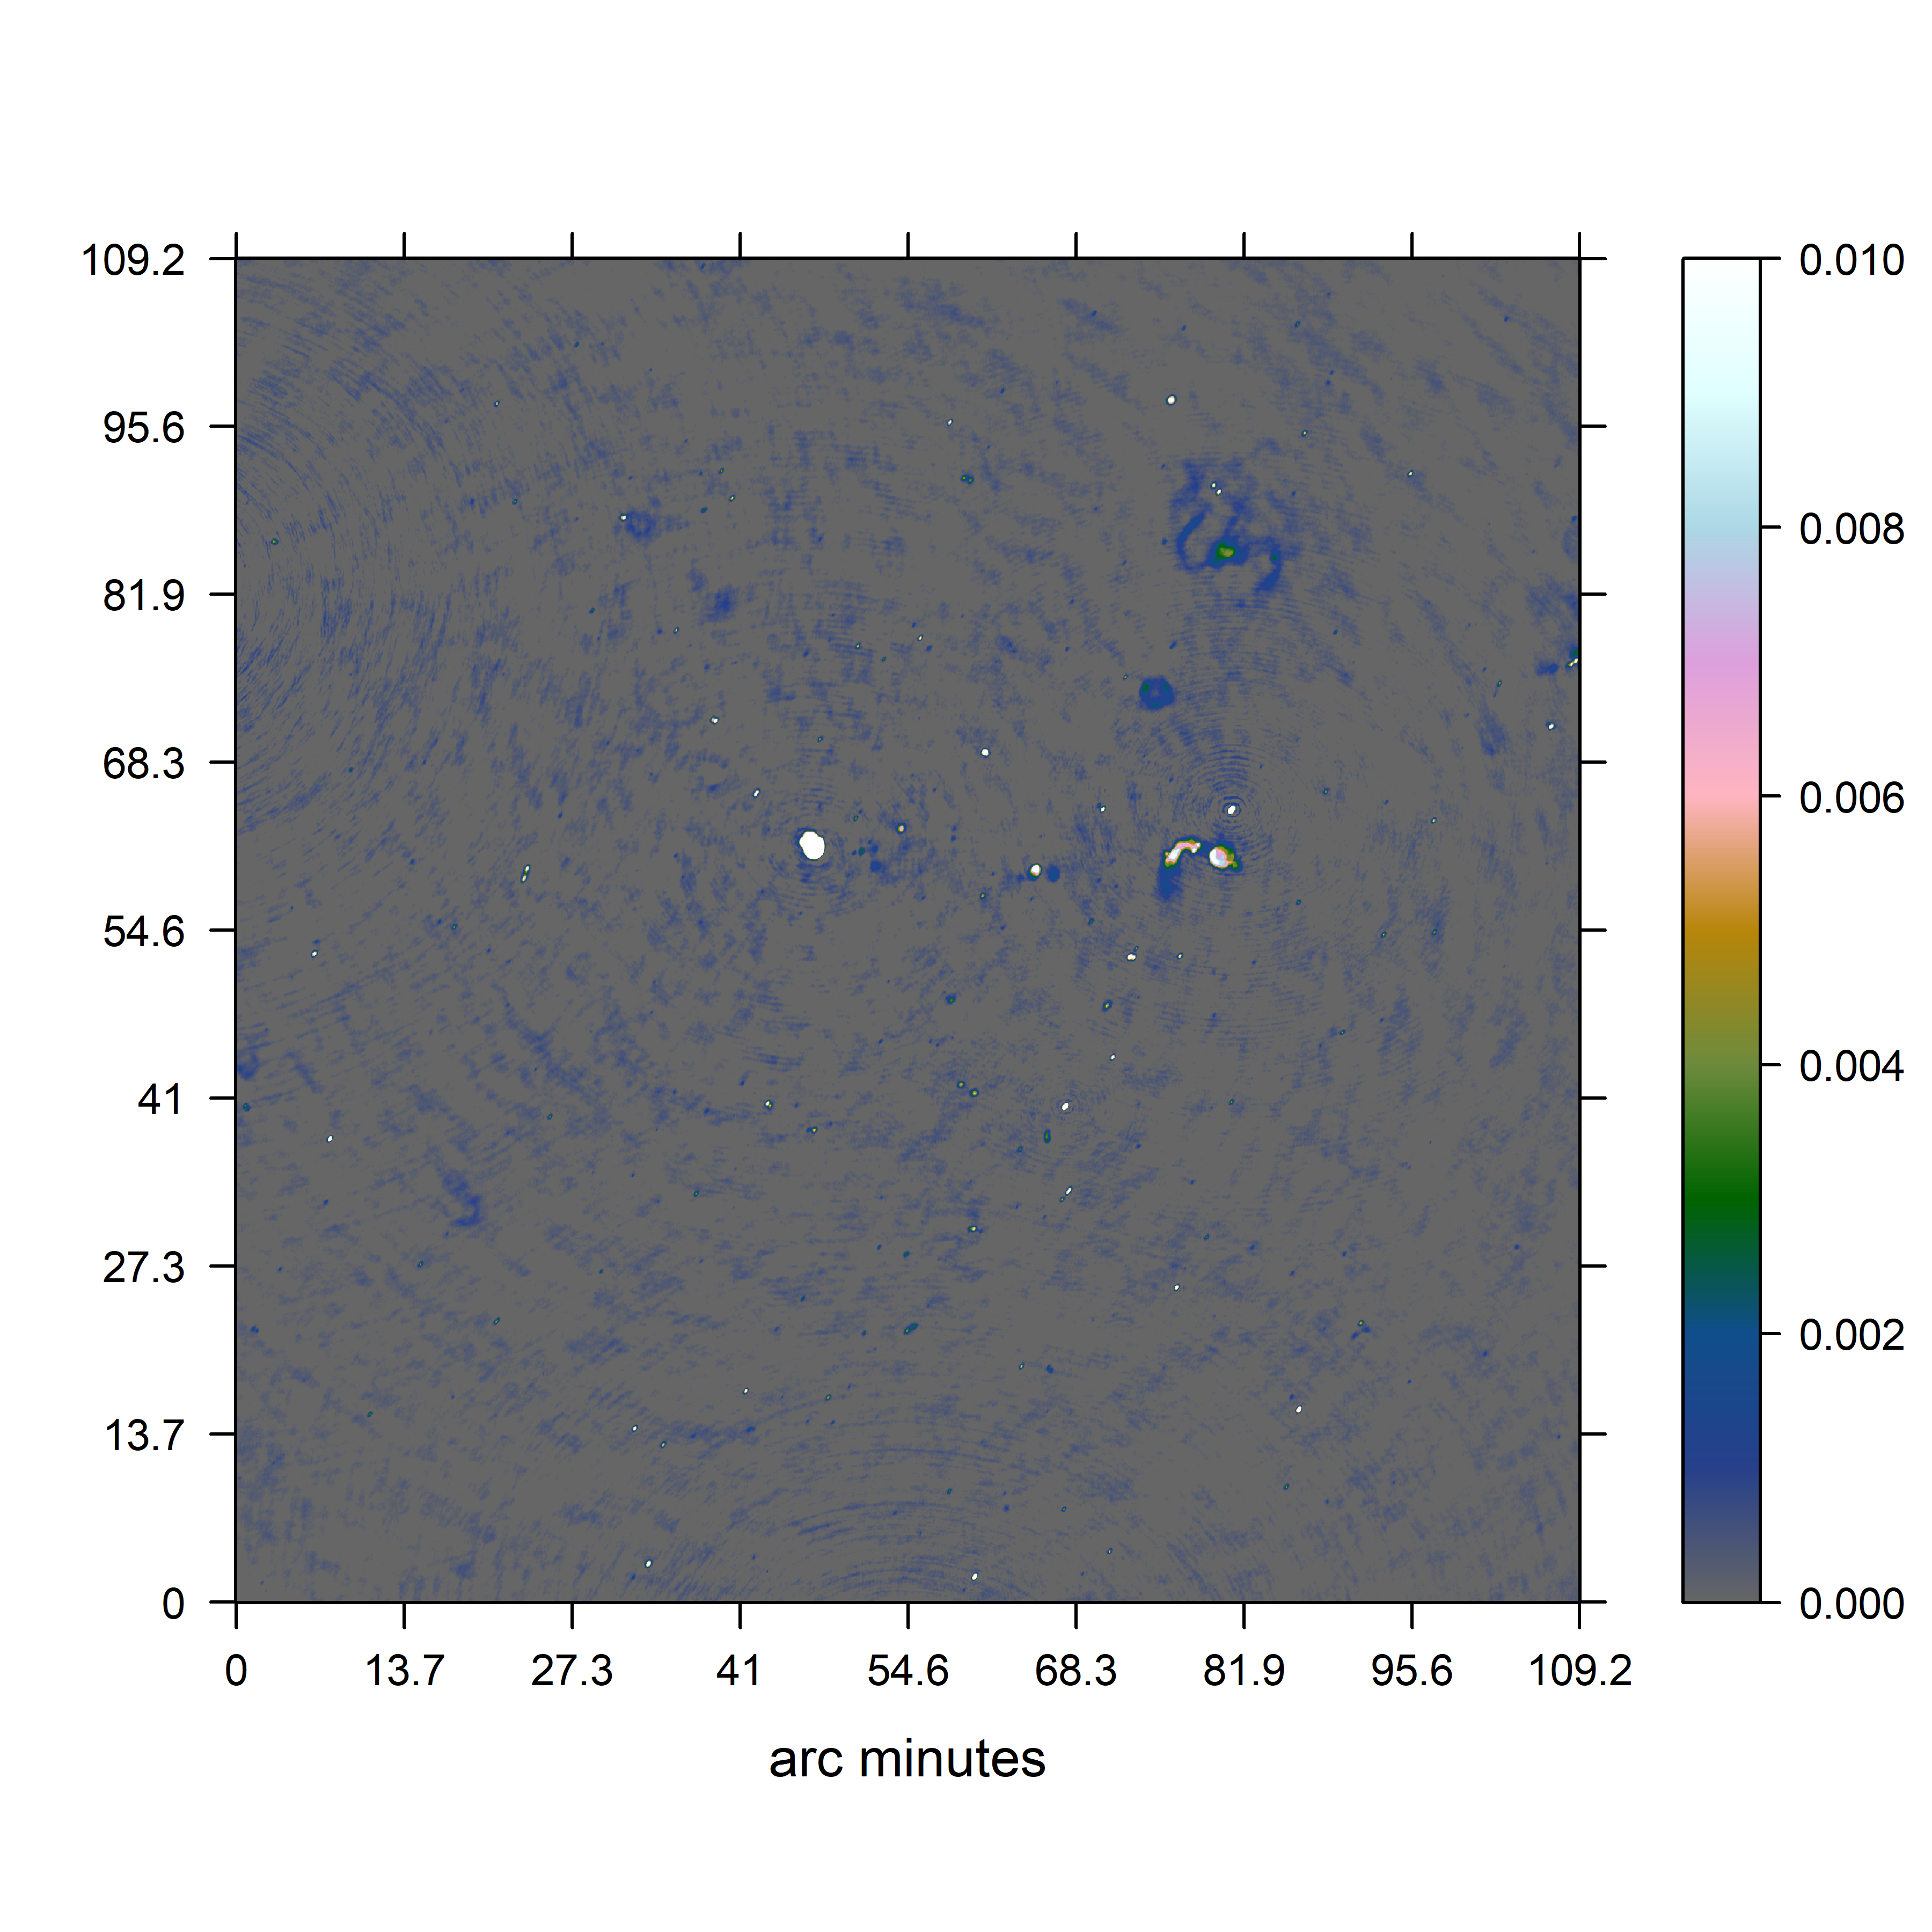
\includegraphics[width=0.6\linewidth]{./chapters/21.scalability/meerkat.png}
	\caption{WSCLEAN Reconstruction of the MeerKAT observation.}
	\label{scale:wsclean}
\end{figure}

Set $J=8$
For Coordinate Descent we need estimates for $S$ and $I_{CD}$. We under-estimate the true values use them from our reconstruction of simulated MeerKAT data \ref{results:mixed:cd}. We it converges within $I_{CD}=10$ iterations, our approach uses $10*J$ iterations.
Favourable assumption for Coordinate Descent. The reconstruction of the MeerKAT image \ref{scale:wsclean} has complex-shaped extended emissions. Approximating those with gaussian-like starlets likely leads to more non-zero starlets than 250.

When we put all values into our cost functions \eqref{results:cd:omega} and \eqref{results:clean:o}, CLEAN arrives at 1.9 times the costs of WSCLEAN. Mind you this is only when we can keep all necessary columns of $F^{-1}$ in our memory, eating up 1.1 terabytes\footnote{If we assume 64 bit floating point accuracy for the real and complex values of the Visibilities.} in our case. If not, the columns have to be re-calculated on the fly, increasing the runtime costs considerably.

Other compressed Sensing approaches. \cite{pratley2018fast} reported 10 Major Cycles for a Compressed Sensing reconstruction on simulated data. If we plug in 10 Major Cycles in the WSCLEAN cost function for a rough estimate, we arrive at Coordinate Descent needing 1.2 the times of other compressed sensing approaches.

Coordinate Descent scales independently of image size.
Pixel to Visibility ratio
Note that the costs scale roughly linear to the pixels per Visibility ratio.
The uncalibrated dataset contains 8 times more Visibilities. Due hardware limitations

The issue with Coordinate Descent's runtime complexity lies in the term $I_{CD} * [S * 4M +\ldots]$ of \eqref{results:cd:omega}, which scales with the "content" of the image $S$, multiplied with the Visibilities. Coordinate Descent cannot afford many iterations nor many non-zero components, because both of these numbers get multiplied together with $M$, the largest number in the problem. With the Major Cycle, WSCLEAN is able to get around this limitation, and scales any content dependant factors on $N$ instead of $M$. 

Indeed, the runtime of our Coordinate Descent algorithm could be improved by using the major cycle architecture, essentially replacing $M$ with $N$ and we arrive at the term $I_{CD} * [S * 4N +\ldots]$. By using the Major Cycle architecture, Coordinate Descent can afford more iterations and more non-zero components in the image for the same runtime complexity. Furthermore $N$ lies on a uniformly sampled grid. We may be able to use the FFT instead of caching columns of $F^{-1}$, and reduce the memory requirement at the same time.



\subsection{Embracing the Major Cycle}
In this project, we created a Compressed Sensing reconstruction which works outside the Major Cycle architecture. With Coordinate Descent as optimization algorithm and starlets as regularization, it does not need the non-uniform FFT during reconstruction. Instead, it uses the relevant columns of the Fourier Transform matrix.  We exploited the starlet regularization for estimating which columns are likely necessary for the reconstruction. This approach naturally extends to the wide field of view measurement equation \eqref{meerkat:ftsphere}. It can handle the $w$-term explicitly and does not need any $w$-term approximation algorithm. To our knowledge, this approach has not been explored previously for radio interferometer image reconstruction. 


Proof-of-concept-implementation, as it is it may not converge to the true minimum. 
On Simulated dataset, it has 
Coordinate Descent created super-resolved point sources on simulated MeerKAT data. Compared to CLEAN, our reconstruction recovered the total flux accurately.

The question is if this approach has the potential to be cheaper than CLEAN. Can compressed sensing reconstructions reduce the runtime costs by getting rid of the Major Cycle. We extrapolated the minimum theoretical costs of our approach to a real-world MeerKAT observation and compared them with WSCLEAN. Sadly, our minimum estimate is approximately twice as expensive as WSCLEAN. 
With this approach, we did not improve upon the runtime costs of Compressed Sensing on large scale reconstructions.

Coordinate Descent costs scale the ratio between Visibilities and pixels. It is more cost effective, the more pixels we have per visibility.
Intuitively, the major cycle reduces the costs, if we have a lot fewer Pixels than Visibilities. In our case, we have approximately 32 more Visibilities than pixels. Our approach scales independently of the image size, but the image size is a far smaller number in the MeerKAT reconstruction problem, which makes the Major Cycle architecture a sensible way to reduce costs. Indeed, our approach can potentially be reduced in costs by using the major cycle, even brush over the large memory requirement.

As it is, our approach does not lead to a runtime cost reduction. However, our apporach is too accurate, we calculate the fourier transform in the area of mere floating-point inaccuracies. Not necessary, the instrument is more inaccurate than that. The Major Cycle exploits this with the non-uniform FFT approximation. Currently, we do it precisely.

Furthermore, we may not need all the Visibilities. Redundant information, can reconstruct the image with a subset of Visibilities. HOpefully self-calibration does not kill this idea.

With both, maybe there is a way to use this approach. It might be end up easier to distribute, because we do not need

Approach with other priors possible.










That does not mean our approach is useless. If we have a reconstruction problem, where 

Scales with the ratio between Visibilities and 

Question if this is the way to scale to large scale reconstruction. Our way is potentially easier to distribute, because it has plain matrix multiplications instead of approximation algorithms.

used an idealized algorithm to estimate the minimum runtime complexity. Turns out it is not competitive to other Major Cycle reconstructions. Each column of the Fourier Matrix has the length of the Visibilities. Massive Memory requirement on top of it.  Sparsity depends on the prior. We could use different priors for reconstruction which may be more sparse, reducing the runtime and need for caching columns. However, the major cycle is just too competitive, we would need a VERY sparse prior in order to have a chance against Major Cycle reconstructions.

Indeed, even our Coordinate Descent algorithm can potentially be sped up with the Major Cycle, potentially getting rid of the massive memory requirement.









 
